\section{Vrai chaos déterministe}
\minitoc
\begin{frame}
  \frametitle{Vrai chaos déterministe}
  \begin{itemize}
  \item générateurs basés sur la \textbf{théorie des nombres}
  	\begin{itemize}
  		\item<2-> séquences périodiques
  		\item<3-> propriétés rendant la suite en partie prévisible : nombres générés dépendants de ceux qui les précédent 
	\end{itemize}
\item

\item<4->
  générateurs basés sur la \textbf{théorie du chaos}
  \begin{itemize}
  \item<5-> séquences imprévisibles
  \item<6-> ...mais peut-être périodiques!
\end{itemize}  
\item

\item<7-> le générateur pseudo-aléatoire de Saito \&
  Yamaguchi (2017) utilise les deux théories
	\end{itemize}   
\end{frame}
\subsection{Décalage de Bernouilli}
\begin{frame}
\frametitle{Point de départ : décalage de Bernoulli}
\begin{center}
{\LARGE $\alpha_{n+1}=(2\alpha_n)\ mod\ 1$\par}
\medskip
définit une suite où $\alpha_n \in [0;1[$.
\end{center}
\onslide<2->{
\par
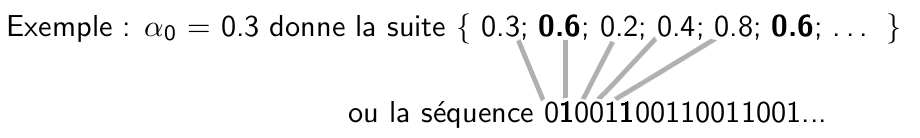
\includegraphics[scale=1]{correspondance.png}}
\medskip
\onslide<3->
\begin{itemize}
\item<3-> si $\alpha_0$ est \textbf{rationnel} $\Rightarrow$ séquence périodique, très prévisible \\
\item<4-> si $\alpha_0$ est \textbf{irrationnel} $\Rightarrow$ séquence  \textbf{non périodique}
\end{itemize}
\onslide<5->{
\medskip
Variation infinitésimale de $\alpha_0 \longrightarrow$ changement radical de la séquence \\}
\onslide<6->{
\begin{center}
 sensibilité aux conditions initiales :\\
 caractéristique d'un processus \textbf{chaotique}
\end{center}}
\end{frame}
\subsection{Sensibilité aux conditions initiales}
\begin{frame}
\definecolor{bleu}{rgb}{0.3,0.5,0.95}
\definecolor{rouge}{rgb}{0.8,0.2,0.2}
\frametitle{décalage de Bernoulli : sensibilité aux conditions initiales}
\begin{minipage}{0.49\textwidth}
 \begin{center}
  {\Large \textcolor{bleu}{$\alpha_0$} = $\frac{\pi}{4}$ \par} 
  \medskip
  irrationnel \\
  $\simeq$ 0.785398\textcolor{bleu}{16}...
 \end{center} 
\end{minipage}
\begin{minipage}{0.49\textwidth}
  \begin{center}
    {\Large \textcolor{rouge}{$\alpha_0$} = $\frac{355}{452}$ \par}
  	\medskip
	rationnel \\
	$\simeq$ 0.785398\textcolor{rouge}{23}...
\end{center}
\end{minipage}
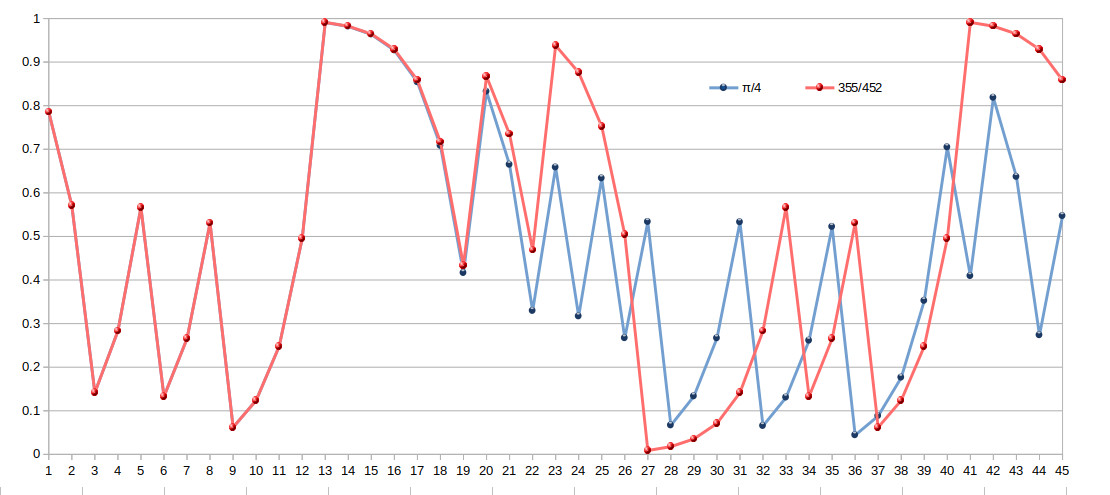
\includegraphics[scale=1.33]{comparaison.png}
\end{frame}
\begin{frame}
\frametitle{décalage de Bernoulli : problème de \definecolor{rouge}{rgb}{0.8,0.2,0.2}
précision}
\begin{minipage}{0.49\textwidth}
 \definecolor{rouge}{rgb}{0.8,0.2,0.2}
  \begin{center}
  nombres réels \\
  précision limitée par la mémoire
 \end{center}
 \medskip
 \begin{tabular}{c c l}
  $\alpha_0$ & = & 0.1100100100001111110110 \\
  $\alpha_1$ & = & 0.100100100001111110110\textcolor{rouge}{0} \\
  $\alpha_2$ & = & 0.00100100001111110110\textcolor{rouge}{00} \\
  $\alpha_3$ & = & 0.0100100001111110110\textcolor{rouge}{000} \\
  ... \\
 \end{tabular} 
 \medskip
\end{minipage}
\onslide<2->{
\begin{minipage}{0.49\textwidth}
  \definecolor{rouge}{rgb}{0.8,0.2,0.2}
  \begin{center}
  \textcolor{rouge}{\textbf{problème}} \\
   éviter la perte d'un bit \\
   à chaque étape \\
  \end{center}
  \medskip
\end{minipage}}
\onslide<3->{
\begin{center}
   comment gérer des \\
   {\Large valeurs exactes\par} 
   pour $\alpha_n$ ? \\
\end{center}}
\end{frame}
\subsection{Racines polynomiales du $3^e$ degré}
\begin{frame}
\frametitle{Racines polynomiales du $3^e$ degré}
Solution de Saito et Yamaguchi (2017)\\
\medskip
 $\alpha_n$  racine unique d’un polynôme du 3e degré :  $f_n(\alpha_n) = 0$ \\
 avec $f_n(x) = x^3+b_n x^2+c_n x+d_n$, et $\epsilon_n = (\alpha_n)$. \\
\onslide<2->{
\medskip
\begin{tabular}{*{6}{c}}
où & $b_n^2-3 c_n \leqslant 0$
& ; & $d_n < 0$
& ; & $1 + b_n + c_n + d_n > 0$
\end{tabular}}
\onslide<3->{ 
\par \medskip
Exemple : $f_0(x) = x^3+x-1$\\
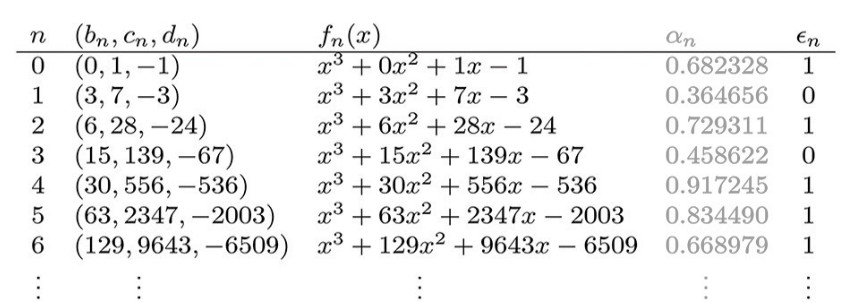
\includegraphics[scale=0.75]{SaitoYamaguchi2017.png}\\ }
\begin{center}
\only<4>{\textbf{$\alpha_{n+1}=2 \alpha_n-\epsilon_n$ permet un calcul simple des coefficients de $f_{n+1}$} \\
(opérations élémentaires)}
\only<5>{$1 + 2b_n + 4c_n + 8d_n < 0 \ \Leftrightarrow \ \alpha_n > \frac{1}{2} \ \Leftrightarrow \ \epsilon_n = 1$ \\
 \textbf{évite le calcul des $\alpha_n$}}
\only<6>{le stockage d'une seule étape demande beaucoup d'\textbf{espace mémoire}\\
complexité en $O(n)$}
\end{center}
\end{frame}
\subsection{Avantages/inconvénients de l'algorithme}
\begin{frame}
\frametitle{Qualité du résultat et utilité de l'algorithme}
\begin{center}
\includegraphics[scale=1]{graphique.png}\\
\end{center}
\begin{itemize}
 \item 
   calcul lent (pas de production on-the-fly)
 \item<2->  
   indépendance (imprévisibilité)
 \item<3->  
   avec un bon choix de $f_0$ ( $c_0$ assez grand et $d_0\geqslant-(b_0+c_0)$ ) \\
   distribution presque uniforme
 \item<4->
   bonne qualité $\rightarrow$ séquences de test statistiques 
\end{itemize} 
\par \medskip
\onslide<5>{
\textbf{Référence} : 
\textit{Pseudorandom number generator based on the Bernoulli map on cubic algebraic integers}, 
Asaki Saito \& Akihiro Yamaguchi, 2017.} 
\end{frame}

